\documentclass[10pt]{article}

% Specify the margins and text size.
\setlength{\textwidth}{6.6in}
\setlength{\textheight}{9.8in}
\setlength{\oddsidemargin}{0pt}
\setlength{\evensidemargin}{0pt}
\setlength{\topmargin}{0pt}
\setlength{\hoffset}{-.05in}
\setlength{\voffset}{-1in}

\setlength{\parskip}{5pt}
\setlength{\parindent}{0pt}

% Load some fonts and symbol packages
\usepackage{latexsym}
\usepackage{pifont}       % contains 'star' symbol for counterinsurgency handbook title
\usepackage{yfonts} 
\usepackage{amsmath}
\usepackage{amsfonts}

\usepackage{graphicx}     % actually, this is loaded by pstricks
\usepackage[T1]{fontenc}
\usepackage{ifthen}
\usepackage{pstricks,pst-grad,pst-text,pst-node,multido,pst-plot,pst-func,calc,pst-3dplot}
%\usepackage[all]{xy}
%\usepackage{animate}

% The hyperref package inserts links into the pdf.
\definecolor{MyLinkColor}{rgb}{.1,.2,1}
\definecolor{MyCiteColor}{rgb}{.1,1,.2}
\definecolor{MyURLColor}{rgb}{.4,.4,.4}
\usepackage[backref=true,pagebackref=false,hyperindex,colorlinks=true,
  linkcolor=MyLinkColor,urlcolor=MyURLColor]{hyperref}


% The tweaklist package is something I found on the web.  It provides a simple interface
% for making changes to spacing used in the itemize and enumerate environments.  Comment
% this out if you don't care to use tweaklist.
\usepackage{tweaklist}
\renewcommand{\itemhook}{\setlength{\parskip}{2pt}\setlength{\parsep}%
{1pt}\setlength{\topsep}{0pt}\setlength{\itemsep}{0pt}}

\newcommand{\U}{\underline{\hspace{5pt}}}

\usepackage{listings}
\newcommand{\Z}{\hphantom{0}}

\newcommand{\HH}{\hspace{10pt}\hphantom{a) } }

\begin{document}
\pagestyle{empty}
\lstset{language=R, showspaces=false, showstringspaces=false}


%%%%%%%%%%%%%%%%%%%%%%%%%%%%%%%%%%%%% VERSION 1 %%%%%%%%%%%%%%%%%%%%%%%%%%%%%%%

\href{http://www.su.edu}{
\includegraphics[height=1.75cm]{sulogo.eps}}
\vspace{-1.69cm}

{{\ }\hfill\small
\begin{tabular}{cl}
& Math 207\\
& Introduction to Statistics\\
\end{tabular}
}
\setlength{\baselineskip}{1.05\baselineskip}

\begin{center}
\textbf{\large  Final Exam}
\end{center}
No books or notes  may be used. You may, however, use a calculator or statistical software (such as R).
\medskip

1. (10 points)  A program is being tested on an extremely expensive computer.  
Due to costs, the program is only run twice.  The output values are $4$ and $8$.
If the  program is running correctly, its average output value is $4$.
Is the program running correctly?  State the statistical test that you use and
compute the test statistic.  Estimate the $P$-value and discuss its significance.
\vspace{3.7in}


2. (10 points)
Suppose 25 readings on the length of a bike trail show an average of 12 miles and  SD
of 50~feet.
%The Bureau of Standards is about to weigh a one-kilogram checkweight 100 times, and take
%the average of the measurements.  They are willing to assume the
%Gauss model, with no bias, and on the basis of past experience they 
%estimate the SD of the error box to be 50 micrograms.
\medskip

\hspace{10pt} a) The average of all 25 measurements is likely to be off
the exact length by \underline{\hspace{1in}} or so.
\vspace{0.7in}
%
%\hspace{20pt} b) The SD of all 100 measurements is likely to be around \underline{\hspace{1in}}.
%\vspace{0.8in}
%\hspace{20pt} b) If you The SD of all 100 measurements is likely to be around \underline{\hspace{1in}}.
%\vspace{0.8in}

\hspace{10pt} b) Esimate the probability that the average of all 25 measurements
will be within 10 feet of the\vspace{-4pt}

\HH exact length.
\vspace{1.2in}

\hspace{10pt} c) Find a 95\% confidence interval on the length  of the trail.

\vfill
\eject


3. (20 points)
A simple random sample of 144 Pittsburgh residents is taken.  
$1/2$~of these residents indicate that they own hybrid-electric vehicles.

\hspace{10pt} a) Find a 95\% confidence interval on the percentage of residents
who own hybrid-electric vehicles.
\vspace{1.5in}

\hspace{10pt} b) Explain what this 95\% confidence interval means (i.e., there is
a 95\% chance of what?).
\vspace{1.5in}


\hspace{10pt} c) Do the data support the null hypothesis that
45\% of the
  Pittsburgh residents own hybrid-electric\vspace{-4pt}

  \HH  vehicles? (i.e., that the observed value differs from 45\% due to chance)?
State the statistical test that\vspace{-4pt}

\HH you use and estimate the $P$-value.
\vspace{2.5in}


\hspace{10pt} d) Suppose you learn that all 144 of the subjects were 
medical administrators.  How might this impact \vspace{-4pt}

\HH your answers to b) and c)?
\vspace{-4pt}

\vfill
\eject
{\ }

4. (10 points) A simple random sample of 64 Winchester residents is taken.
$1/5$ of these residents indicate that they own hybrid-electric vehicles.
Use this data and the data from \#3 to 
test the hypothesis that the proportions of Winchester and Pittsburgh residents  who
own hybrid-electric vehicles are the same.
Estimate the $P$-value and discuss its significance.
\vspace{4in}

5. (10 points) A coin is to be flipped 13 times. What is the chance of 
getting exactly 11 heads?  Simplify your answer as much as possible.
What is the chance of getting at least 11 heads?
\vfill
\eject
{\ }

6. (15 points) Data is collected for the age (in days) and circumference (in millimeters) 
of orange trees.
The following statistics summarize the data
\begin{align*}
\mbox{average age}&= 900\;\mbox{days} & \mbox{SD}_{\scriptsize\mbox{days}} &= 500\;\mbox{days}\\
\mbox{average circumference} &= 120\;\mbox{mm} & \mbox{SD}_{\scriptsize\mbox{circ}}\; &= 60\;\mbox{mm}
   & r=0.7
\end{align*}

\begin{center}
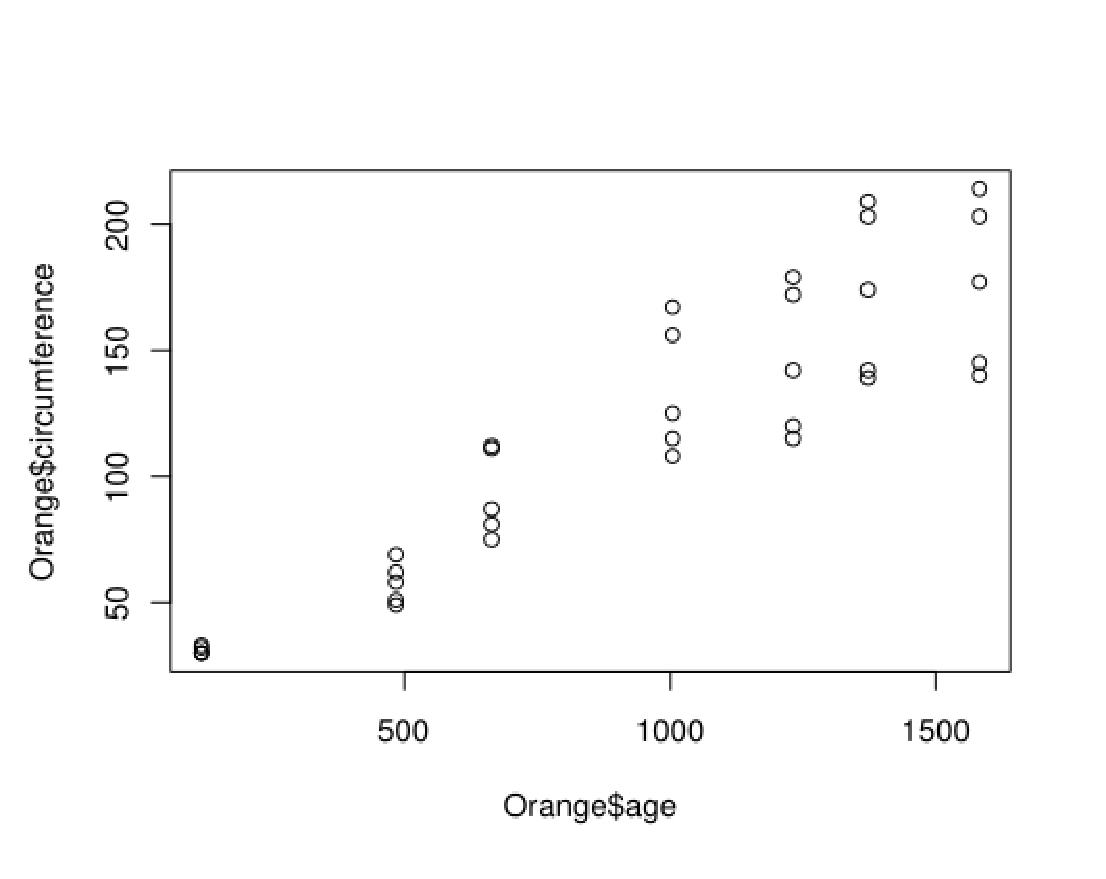
\includegraphics[height=2.5in,bb= 0 0 515 335, clip]{Oranges.eps}
\end{center}

\hspace{10pt} a) Find a formula for the regression line to predict circumference 
from age.  Sketch the line in the\vspace{-4pt}

\HH  figure above.
\vspace{1.5in}

\hspace{10pt} b) Estimate the circumference of an orange tree that is
1035 days old.
\vspace{2in}

\hspace{10pt} c) About 68\% of the orange trees that are 1035 days old 
have what range of circumferences?
\vfill
\eject
{\ }

7. (5 points)
Suppose that you take a large number of independent random samples from a box of numbered
tickets.
Fill in the blanks.

\begin{itemize}
\item[a)] The histogram of the averages of the samples will
  will look approximately like a \underbar{\hspace{1.2in}}.\vspace{.4in}
\item[b)] The histogram of the sums of the  samples will
  will look approximately like a \underbar{\hspace{1.2in}}.\vspace{.4in}
  
\item[c)] Suppose that the tickes are all 0s and 1s.  The histogram of the
  percent of 1s in the  samples will
  will look approximately like a \underbar{\hspace{1.2in}}.
\end{itemize}
\vspace{1in}

8. (5 points) 1. A fair die is rolled 10 times.  The number of dots showing on the rolls
was:  2, 1, 4, 4, 2, 4, 1, 3, 1, 5. 
Draw a histogram of this data.
\vspace{1.5in}

9.  (15 points) An experiment consists of rolling a die 400 times and recording how often
the die shows an even number.

\hspace{10pt} a) Write down a box model to represent the experiment.
\vspace{.5in}

\hspace{10pt} b) Compute the mean and SD of the box.
\vspace{1in}

\hspace{10pt} c) The number of times that the die will show an even number 
will be around \underline{\hspace{1in}},\vspace{10pt}

\hspace{10pt}\hphantom{e) }give or take \underline{\hspace{1in}} or so.  %Justify your answers.
\vspace{.8in}

\hspace{10pt} d) The chance that the percent of times will be between 45\% and 55\% is about
\underline{\hspace{1in}} \%.  
\vfill
\eject

\begin{center}
\textbf{\large Formula Sheet}
\end{center}\vspace{-15pt}
\begin{align*}
\mbox{mean} &=\frac{1}{n}\left(x_1 + \cdots + x_n\right)\\[5pt]
\mbox{SD}   &=\sqrt{\frac{1}{n}\left( (x_1 - \mbox{mean})^2 + \cdots + (x_n - \mbox{mean})^2\right)}\\[10pt]
\mbox{sd}   &=\sqrt{\frac{1}{n-1}\left( (x_1 - \mbox{mean})^2 + \cdots + (x_n - \mbox{mean})^2\right)}\\[10pt]
%
\mbox{EV}_{\mbox{\footnotesize sum}} & = n\,\mbox{AV}_{\mbox{\footnotesize box}}\\
\mbox{SE}_{\mbox{\footnotesize sum}} & = \sqrt{n}\;\;\mbox{SD}_{\mbox{\footnotesize box}}\\[10pt]
%
\mbox{EV}_{\mbox{\footnotesize av}} & = \mbox{AV}_{\mbox{\footnotesize box}}\\
\mbox{SE}_{\mbox{\footnotesize av}} & = \mbox{SD}_{\mbox{\footnotesize box}}\,\big{/}\sqrt{n}\\[10pt]
%
%\mbox{EV}_{\mbox{\footnotesize \%}} & = \mbox{AV}_{\mbox{\footnotesize box}}\\
%\mbox{SE}_{\mbox{\footnotesize \%}} & = \mbox{SD}_{\mbox{\footnotesize box}}\,\big{/}\sqrt{n}\\[5pt]
%
\noalign{Shortcut formula (if there are only two different kinds of numbers in the box):}
\mbox{SD}_{\mbox{\footnotesize box}} &=
  \left(\mbox{big \#} - \mbox{small \#}\right)\,\sqrt{
  \left(\begin{array}{c}\mbox{fraction of}\\ \mbox{tickets with the}\\ \mbox{big number}\end{array}\right)
  \left(\begin{array}{c}\mbox{fraction of}\\\mbox{tickets with the}\\\mbox{small number}\end{array}\right)}\\
%
\mbox{95\% confidence interval} &= \mbox{observed} \;\pm\; 2\,\mbox{SE}\\[5pt]
z &= \frac{\mbox{observed} - \mbox{expected}}{\mbox{standard error}}\\[10pt]
%
\noalign{Regression line:}
y - y_{\mbox{\footnotesize av}} &= r\,\frac{\mbox{\footnotesize sd}_y}{\mbox{\footnotesize sd}_x}\,
       \left(x - x_{\mbox{\footnotesize av}}\right)\\[5pt]
\noalign{RMS error for the regression line:}
\mbox{RMS}_{\mbox{\footnotesize reg}} &= \mbox{sd}_y\,\sqrt{1 - r^2}\\[10pt]
\noalign{Binomial Formula:}
&{} \frac{n!}{k!\,(n-k)!},p^k\,(1-p)^{n-k}
\end{align*}

\vfill
\eject

%%%%%%%%%%%%%%%%%%%%%%%%%%%%%%%%%%%%% VERSION 2


\href{http://www.su.edu}{
\includegraphics[height=1.75cm]{sulogo.eps}}
\vspace{-1.69cm}

{{\ }\hfill\small
\begin{tabular}{cl}
& Math 207\\
& Introduction to Statistics\\
\end{tabular}
}

\begin{center}
\textbf{\large  Final Exam}
\end{center}
No books or notes  may be used. You may, however, use a calculator or statistical software (such as R).
\medskip

1. (10 points)  A program is being tested on an extremely expensive computer.  
Due to costs, the program is only run twice.  The output values are $1$ and $5$.
If the  program is running correctly, its average output value is $1$.
Is the program running correctly?  State the statistical test that you use and
compute the test statistic.  Estimate the $P$-value and discuss its significance.
\vspace{3.7in}


2. (10 points)
Suppose 16 readings on the length of a bike trail show an average of 8 miles and  SD
of 60~feet.
%The Bureau of Standards is about to weigh a one-kilogram checkweight 100 times, and take
%the average of the measurements.  They are willing to assume the
%Gauss model, with no bias, and on the basis of past experience they 
%estimate the SD of the error box to be 50 micrograms.
\medskip

\hspace{10pt} a) The average of all 16 measurements is likely to be off
the exact length by \underline{\hspace{1in}} or so.
\vspace{0.7in}
%
%\hspace{20pt} b) The SD of all 100 measurements is likely to be around \underline{\hspace{1in}}.
%\vspace{0.8in}
%\hspace{20pt} b) If you The SD of all 100 measurements is likely to be around \underline{\hspace{1in}}.
%\vspace{0.8in}

\hspace{10pt} b) Esimate the probability that the average of all 16 measurements
will be within 30 feet of the\vspace{-4pt}

\HH exact length.
\vspace{1.2in}

\hspace{10pt} c) Find a 95\% confidence interval on the length  of the trail.

\vfill
\eject


3. (20 points)
A simple random sample of 225 Pittsburgh residents is taken.  
$1/2$~of these residents indicate that they own hybrid-electric vehicles.

\hspace{10pt} a) Find a 95\% confidence interval on the percentage of residents
who own hybrid-electric vehicles.
\vspace{1.5in}

\hspace{10pt} b) Explain what this 95\% confidence interval means (i.e., there is
a 95\% chance of what?).
\vspace{1.5in}


\hspace{10pt} c) Do the data support the null hypothesis that
45\% of the
  Pittsburgh residents own hybrid-electric\vspace{-4pt}

  \HH  vehicles? (i.e., that the observed value differs from 45\% due to chance)?
State the statistical test that\vspace{-4pt}

\HH you use and estimate the $P$-value.
\vspace{2.5in}


\hspace{10pt} d) Suppose you learn that all 225 of the subjects were 
medical administrators.  How might this impact \vspace{-4pt}

\HH your answers to b) and c)?
\vspace{-4pt}

\vfill
\eject
{\ }

4. (10 points) A simple random sample of 144 Winchester residents is taken.
$2/5$ of these residents indicate that they own hybrid-electric vehicles.
Use this data and the data from \#3 to 
test the hypothesis that the proportions of Winchester and Pittsburgh residents  who
own hybrid-electric vehicles are the same.
Estimate the $P$-value and discuss its significance.
\vspace{4in}

5. (10 points) A coin is to be flipped 12 times. What is the chance of 
getting exactly 11 heads?  Simplify your answer as much as possible.
What is the chance of getting at least 11 heads?
\vfill
\eject
{\ }

6. (15 points) Data is collected for the age (in days) and circumference (in millimeters) 
of orange trees.
The following statistics summarize the data
\begin{align*}
\mbox{average age}&= 900\;\mbox{days} & \mbox{SD}_{\scriptsize\mbox{days}} &= 500\;\mbox{days}\\
\mbox{average circumference} &= 120\;\mbox{mm} & \mbox{SD}_{\scriptsize\mbox{circ}}\; &= 60\;\mbox{mm}
   & r=0.8
\end{align*}

\begin{center}
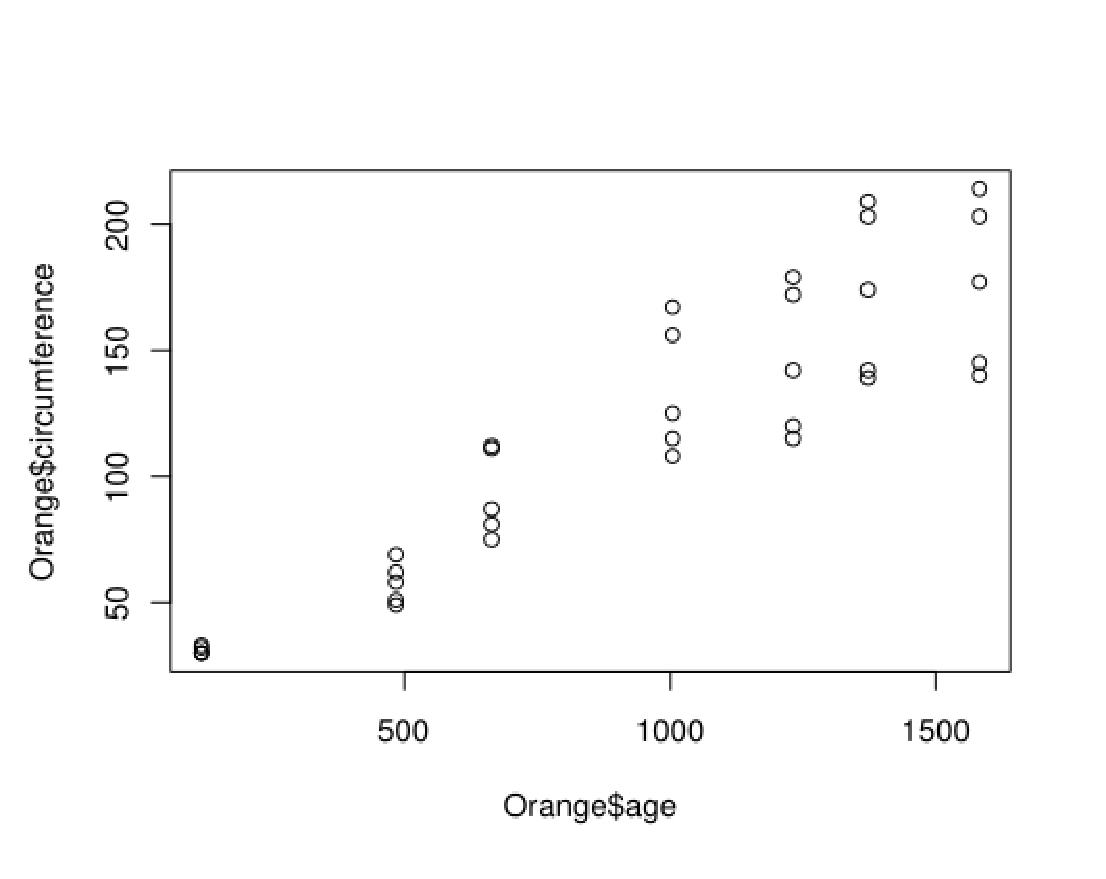
\includegraphics[height=2.5in,bb= 0 0 515 335, clip]{Oranges.eps}
\end{center}

\hspace{10pt} a) Find a formula for the regression line to predict circumference 
from age.  Sketch the line in the\vspace{-4pt}

\HH  figure above.
\vspace{1.5in}

\hspace{10pt} b) Estimate the circumference of an orange tree that is
1000 days old.
\vspace{2in}

\hspace{10pt} c) About 68\% of the orange trees that are 1000 days old 
have what range of circumferences?
\vfill
\eject
{\ }

7. (5 points)
Suppose that you take a large number of independent random samples from a box of numbered
tickets.
Fill in the blanks.

\begin{itemize}
\item[a)] The histogram of the averages of the samples will
  will look approximately like a \underbar{\hspace{1.2in}}.\vspace{.4in}
\item[b)] The histogram of the sums of the  samples will
  will look approximately like a \underbar{\hspace{1.2in}}.\vspace{.4in}
  
\item[c)] Suppose that the tickes are all 0s and 1s.  The histogram of the
  percent of 1s in the  samples will
  will look approximately like a \underbar{\hspace{1.2in}}.
\end{itemize}
\vspace{1in}

8. (5 points) 1. A fair die is rolled 10 times.  The number of dots showing on the rolls
was:  2, 1, 3, 4, 2, 4, 1, 3, 6, 5. 
Draw a histogram of this data.
\vspace{1.5in}

9.  (15 points) An experiment consists of rolling a die 144 times and recording how often
the die shows an even number.

\hspace{10pt} a) Write down a box model to represent the experiment.
\vspace{.5in}

\hspace{10pt} b) Compute the mean and SD of the box.
\vspace{1in}

\hspace{10pt} c) The number of times that the die will show an even number 
will be around \underline{\hspace{1in}},\vspace{10pt}

\hspace{10pt}\hphantom{e) }give or take \underline{\hspace{1in}} or so.  %Justify your answers.
\vspace{.8in}

\hspace{10pt} d) The chance that the percent of times will be between 45\% and 55\% is about
\underline{\hspace{1in}} \%.  
\vfill
\eject

\begin{center}
\textbf{\large Formula Sheet}
\end{center}\vspace{-15pt}
\begin{align*}
\mbox{mean} &=\frac{1}{n}\left(x_1 + \cdots + x_n\right)\\[5pt]
\mbox{SD}   &=\sqrt{\frac{1}{n}\left( (x_1 - \mbox{mean})^2 + \cdots + (x_n - \mbox{mean})^2\right)}\\[10pt]
\mbox{sd}   &=\sqrt{\frac{1}{n-1}\left( (x_1 - \mbox{mean})^2 + \cdots + (x_n - \mbox{mean})^2\right)}\\[10pt]
%
\mbox{EV}_{\mbox{\footnotesize sum}} & = n\,\mbox{AV}_{\mbox{\footnotesize box}}\\
\mbox{SE}_{\mbox{\footnotesize sum}} & = \sqrt{n}\;\;\mbox{SD}_{\mbox{\footnotesize box}}\\[10pt]
%
\mbox{EV}_{\mbox{\footnotesize av}} & = \mbox{AV}_{\mbox{\footnotesize box}}\\
\mbox{SE}_{\mbox{\footnotesize av}} & = \mbox{SD}_{\mbox{\footnotesize box}}\,\big{/}\sqrt{n}\\[10pt]
%
%\mbox{EV}_{\mbox{\footnotesize \%}} & = \mbox{AV}_{\mbox{\footnotesize box}}\\
%\mbox{SE}_{\mbox{\footnotesize \%}} & = \mbox{SD}_{\mbox{\footnotesize box}}\,\big{/}\sqrt{n}\\[5pt]
%
\noalign{Shortcut formula (if there are only two different kinds of numbers in the box):}
\mbox{SD}_{\mbox{\footnotesize box}} &=
  \left(\mbox{big \#} - \mbox{small \#}\right)\,\sqrt{
  \left(\begin{array}{c}\mbox{fraction of}\\ \mbox{tickets with the}\\ \mbox{big number}\end{array}\right)
  \left(\begin{array}{c}\mbox{fraction of}\\\mbox{tickets with the}\\\mbox{small number}\end{array}\right)}\\
%
\mbox{95\% confidence interval} &= \mbox{observed} \;\pm\; 2\,\mbox{SE}\\[5pt]
z &= \frac{\mbox{observed} - \mbox{expected}}{\mbox{standard error}}\\[10pt]
%
\noalign{Regression line:}
y - y_{\mbox{\footnotesize av}} &= r\,\frac{\mbox{\footnotesize sd}_y}{\mbox{\footnotesize sd}_x}\,
       \left(x - x_{\mbox{\footnotesize av}}\right)\\[5pt]
\noalign{RMS error for the regression line:}
\mbox{RMS}_{\mbox{\footnotesize reg}} &= \mbox{sd}_y\,\sqrt{1 - r^2}\\[10pt]
\noalign{Binomial Formula:}
&{} \frac{n!}{k!\,(n-k)!},p^k\,(1-p)^{n-k}
\end{align*}

\vfill
\eject



\end{document}

